\documentclass[12pt]{article}

\usepackage[utf8]{inputenc}
%\usepackage[T1]{fontenc}

\usepackage{geometry}
\geometry{a4paper}
\usepackage{graphicx}
\usepackage{float}
\usepackage[italian]{babel}

\usepackage{subcaption}

%
%%%%%%%%%%%%%%%%%%%%%%%%%%%%%%%%%%%%%%%%%comando per la gestione semplificata di quotes
\newcommand{\quotes}[1]{``#1''}

%
%%%%%%%%%%%%%%%%%%%%%%%%%%%%%%%%%%%%%%%%%libreria per l'inserimento di link nella
%   bibliografia
\PassOptionsToPackage{hyphens}{url}\usepackage[hidelinks]{hyperref}

\linespread{1.2}
\setlength{\parindent}{0pt}

\begin{document}

%----------------------------------------------------------------------------------------
%	TITOLO
%----------------------------------------------------------------------------------------

\begin{titlepage}

\newcommand{\HRule}{\rule{\linewidth}{0.5mm}}

\center

\textsc{\Large Relazione di progetto di \quotes{Smart City e Tecnologie Mobili}}\\[0.5cm]

\HRule \\[0.4cm]
{
	\huge \bfseries
	Rilevatore di sonnolenza\\
	all'interno di un autoveicolo con\\
	Raspberry Pi\\[0.4cm]
}
\HRule \\[1.5cm]

\vfill

\begin{flushleft}
\emph{Numero del gruppo:}\\
62\\[1cm]
\emph{Componenti del gruppo:}\\
Giacomo Frisoni\\
Marcin Pabich\\[3cm]
\end{flushleft}



\end{titlepage}

%----------------------------------------------------------------------------------------
%	INDICE
%----------------------------------------------------------------------------------------

\tableofcontents

\newpage

%----------------------------------------------------------------------------------------
%	INTRODUZIONE
%----------------------------------------------------------------------------------------

\section{Introduzione}

Il deterioramento delle capacità alla guida causato da sonnolenza è noto per essere uno dei fattori che contribuiscono maggiormente alla formazione di incidenti automobilistici. Secondo un sondaggio del 2011 realizzato dalla National Sleep Foundation sulla popolazione americana, circa il 30\% degli incidenti su strada è dovuto all'affaticamento del conducente e tale dato tende a crescere di anno in anno\cite{SleepInAmerica}. Una recente indagine svolta dalla NHTSA\footnote{NHTSA. National Highway Traffic Safety Administration.} ha inoltre stimato un numero complessivo di 90.000 incidenti in America segnalati dalla polizia nel 2015 (con 41.000 feriti e più di 800 morti), aventi come causa l'insorgere di uno stato di sonnolenza\cite{NHTSA}.\\
La sonnolenza costituisce nello specifico una fase di transizione nel ciclo sonno-veglia, determinante uno stato di torpore e una riduzione del livello di coscienza della persona. Nell'ambito in esame, la sonnolenza deteriora le prestazioni del guidatore e può infine portare all'incapacità di resistere al sonno al volante. Essa può essere dovuta a diversi fattori: condizioni di guida avverse, traffico intenso, alti carichi di lavoro, scarso riposo, orari notturni, disturbi del sonno, abuso di alcol e assunzione di medicinali sono solo alcuni esempi. Tutti questi fattori hanno effetti cumulativi e una loro combinazione può aumentare in modo sostanziale il rischio di incidenti stradali. Gli aspetti critici su cui impatta la sonnolenza alla guida, invece, sono i tempi di reazione, la vigilanza, il livello di attenzione e la velocità nell'elaborare le informazioni.\\
A partire dal 1995 i ricercatori hanno iniziato a concentrare i propri sforzi sulla costruzione di dispositivi di allarme, come una tra le principali tecniche di contromisura. L'obiettivo di questi sistemi è quello di allarmare o risvegliare i conducenti che sono assonnatti o addormentati, riducendo conseguentemente la percentuale di scontri e avvenimenti inattesi sul suolo stradale. Una carenza intrinseca in tutti i tipi di dispositivi di allarme, tuttavia, è da ricercarsi nel fatto che molte persone continuano a guidare anche quando sanno di essere sonnolenti, lottando per rimanere svegli. Sebbene un dispositivo di allarme efficace possa prevenire un incidente, un autista che si addormenta una volta rischia di addormentarsi nuovamente a meno che non smetta di guidare. Da diversi anni gli esperti di sicurezza hanno espresso preoccupazione sul fatto che i dispositivi di allarme possano fornire ai conducenti un falso senso di sicurezza, incoraggiandoli a guidare per lungo tempo\cite{DrowsyDrivingReport}.\\
Il progetto descritto in questo documento si pone l'obiettivo di realizzare un sistema a basso costo, affidabile e non intrusivo per il riconoscimento della stanchezza del conducente in tempo reale, svolgendo un monitoraggio video sul suo volto e applicando tecniche di Computer Vision sui frame catturati. L'implementazione della soluzione si basa sull'uso di un \textit{Raspberry Pi 3 B}, un single-board computer noto per le sue caratteristiche prestazionali rapportate al prezzo e alle dimensioni che lo contraddistinguono.\\
Il sistema acquisisce le immagini dell'utente per mezzo di una camera installata nell'automobile e posizionata frontalmente a esso. La sonnolenza del guidatore è successivamente calcolata in riferimento a una misura comportamentale incentrata sulla chiusura degli occhi (stimata quantitativamente con metodologia \textit{EAR}\footnote{EAR. Eye Aspect Ratio.}\cite{EAR}). A fronte di una chiusura degli occhi protrattasi oltre un tempo definito, il sistema riproduce un allarme per mezzo di un buzzer acustico al fine di reclamare l'attenzione dell'utente ed evidenziare il potenziale pericolo che sta incorrendo.\\
Le principali tecnologie adottate sono \textit{Python} a livello di linguaggio di programmazione, \textit{OpenCV}\cite{OpenCV} come libreria per la manipolazione di foto e video, \textit{dlib}\cite{Dlib} per quanto concerne gli algoritmi di machine learning per l'individuazione e la localizzazione di facial landmark.\\
Il contributo tecnologico/scientifico apportato dal gruppo con l'elaborato in esame si riferisce allo studio e al confronto prestazionale delle varie soluzioni che possono essere implementate, specie in relazione ai limiti dell'hardware adottato. Una particolare attenzione è riposta nelle tecniche di riconoscimento facciale: esse rappresentano la base dell'intero processo e sono note per essere l'elemento centrale sia per la determinazione dell'efficacia del sistema nei vari scenari d'uso che per la sua reale efficienza.

\iffalse
Esporre l’obiettivo del progetto dandone una visione complessiva.\\
Devono essere illustrate le caratteristiche salienti del progetto; deve essere chiara la distinzione tra le tecnologie usate/assemblate durante lo svolgimento dell’elaborato e il contributo tecnologico/scientifico effettivamente apportato dal gruppo.\\

Vincoli circa la lunghezza della sezione (escluse didascalie, tabelle, testo nelle immagini, schemi):

\vspace{1cm}
\begin{tabular}{l|rr}
	& Numero minimo di battute & Numero massimo di battute \\
	\hline
	1 componente & 2000 & 3000 \\
	2 componenti & 2500 & 4500 \\
	3 componenti & 3000 & 6000 \\
	\hline
\end{tabular}
\fi

\newpage


%----------------------------------------------------------------------------------------
%	STATO DELL'ARTE
%----------------------------------------------------------------------------------------

\section{Stato dell'arte}

Misurare direttamente il livello di sonnolenza è complesso. Esistono tuttavia numerosi metodi indiretti capaci di rilevare aspetti correlati e che oggi costituiscono la base per i vari sistemi disponibili sul mercato.
In questa sezione si riportano le soluzioni presenti in letteratura per quanto concerne il problema in esame, distinguendole sulla base del tipo di misura su cui si basano (riassunte in Figura \ref{fig:StateOfTheArt}). Inoltre si citano quelle già operative sul mercato: lo sviluppo di tecnologie per il rilevamento di sonnolenza, infatti, costituisce una sfida sia accademica che industriale.

\subsection{Misure fisiologiche}

Le misure di segnali fisiologici comprendono tecniche quali ECG (elettrocardiogramma), EOG (elettrooculogramma), EEG (elettroencefalogramma) e HRV\footnote{HRV. Heart Rate Variability.}.
Il segnale EEG, in particolare, è il più utilizzato nella classe fisiologica per la misurazione della stanchezza. Esso fornisce informazioni sull'attività del cervello e consente pertanto di individuare la perdita di concentrazione e il rallentamento dei tempi di risposta tipici di chi è affetto da affaticamento e sonnolenza. Il segnale EEG ha varie bande di frequenza: \textit{delta} (0,5-4 Hz) - corrispondente al sonno, \textit{theta} (4-8 Hz) - legata alla stanchezza, \textit{alpha} (8-13 Hz) - rappresentante uno stato di rilassamento e creatività, \textit{beta} (13-25 Hz) - corrispondente a uno stato di vigilanza. Una diminuzione della variazione di potenza nella banda di frequenza \textit{alpha} e un relativo aumento in \textit{theta} è pertanto indice di sonnolenza. Secondo uno studio condotto nel 2011\cite{EEG}, le tecniche EEG sono le più accurate, con un tasso di precisione superiore al 90\%. Tuttavia, le misure fisiologiche faticano a essere adottate nella realtà a causa dei loro costi, della connessione fisica che richiedono con l'autista e dello stress indotto tipicamente nell'utente che indossa le apparecchiature di monitoraggio necessarie. Una soluzione più pratica è stata studiata per Jaguar Land Rover\cite{Jaguar}.

\subsection{Misure basate sul veicolo}

La maggior parte delle soluzioni attualmente disponibili e impiegate dalle case automobilistiche riguardano misure basate sul veicolo e comprendono pertanto l'individuazione di scostamenti rispetto alla propria corsia, la pressione esercitata sui pedali e il movimento delle ruote sterzanti. Si tratta dunque di approcci basati su modelli di guida che hanno lo svantaggio di dipendere fortemente dalle caratteristiche del veicolo, dalle condizioni della strada e dalle capacità del conducente.\\
In un paper del 2009\cite{SWM} un gruppo di ricercatori ha rilevato il livello di sonnolenza con un'accuratezza dell'86\%, considerando le correlazioni tra le micro-regolazioni esercitate sul volante per il mantenimento dell'automobile (individuate grazie a sensori per la misurazione dell'angolo di sterzata) in corsia e l'affaticamento del guidatore stesso. Tale tecnica di rilevamento è denominata SWM\footnote{SWM. Steering Wheel Movement.}.\\
Un'altra misura basata sul veicolo spesso utilizzata per misurare la sonnolenza del conducente è SDLP\footnote{SLDP. Standard Deviation of Lane Position.}, dove la posizione della corsia viene tracciata per mezzo di una telecamera esterna. Il principale limite di questa tecnica risiede nella dipendenza da fattori quali la segnaletica orizzontale, l'illuminazione e le condizioni climatiche.\\
I sistemi implementati oggi all'interno delle automobili di fascia alta tengono in genere conto di un insieme di parametri. Il Driver Alert di Ford\cite{Ford}, il Safety-IBuzz Fatigue Alert di Skoda\cite{Skoda} e il Bosch Driver Drowsiness Detection System\cite{Bosch} adottato da Volkswagen sono i più conosciuti esempi industriali.

\subsection{Misure comportamentali}

Le soluzioni basate su misure di tipo comportamentale sono le più diffuse negli ultimi anni. Esse si basano sulle caratteristiche tipiche del movimento facciale nelle persone assonnate: rapidi e costanti battiti di ciglia, chiusura degli occhi, annuenza o oscillazione della testa e frequenti sbadigli. La maggior parte degli studi pubblicati sugli approcci comportamentali per la determinazione della sonnolenza si focalizza sul battito di ciglia. Sotto questo punto di vista, la misura del PERCLOS\footnote{PERCLOS. Percentuale di chiusura della palpebra sopra la pupilla nel tempo. Riflette la tipica chiusura rallentata degli occhi nei soggetti affetti da sonnolenza.} costituisce la tecnica più diffusa e impiegata anche nell'ambito dei prodotti commerciali.\\
Il principale limite legato all'uso di tecniche di Computer Vision per l'estrazione di feature facciali è l'illuminazione. Le camere normali non consentono di ottenere risultati soddisfacenti in scenari notturni. Per ovviare il problema, alcuni ricercatori hanno fatto uso di una illuminazione infrarossi tramite LED\footnote{LED. Light Emitting Node.}\cite{IEEE} (che consente buone prestazioni di notte ma è meno robusta durante il giorno). Le immagini vengono acquisite dalla camera a un certo frame rate, elaborate per garantire prima l'estrazione del volto e poi per localizzare la specifica regione d'interesse (ad esempio tramite Haar Cascade Classifier o HOG) su cui realizzare il calcolo della misura scelta. Approcci più recenti, infine, si basano su Deep Learning.

\begin{figure}
	\begin{subfigure}{.4\textwidth}
		\centering
		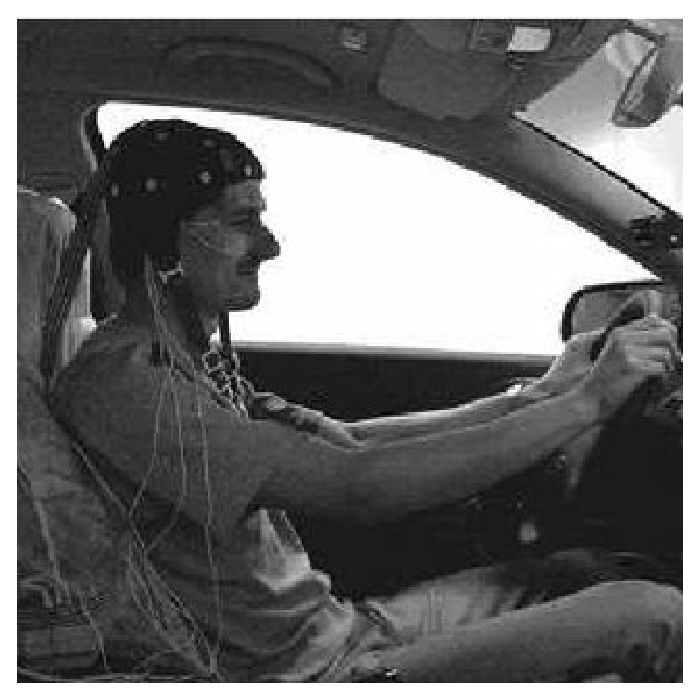
\includegraphics[width=.8\linewidth]{eps/eeg.eps}
		\caption{Esempio pratico di misura fisiologica con casco EEG.}
	\end{subfigure}
	\hspace{5mm}
	\begin{subfigure}{.55\textwidth}
		\centering
		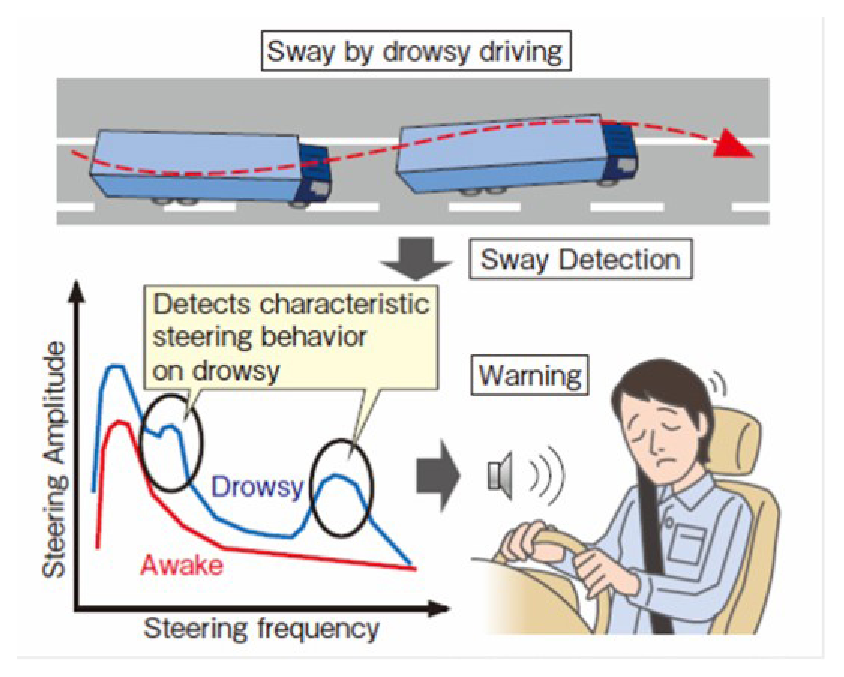
\includegraphics[width=.8\linewidth]{eps/swm.eps}
		\caption{Funzionamento della misura SWM\\basata sul veicolo.}
	\end{subfigure}
	\par\bigskip % force a bit of vertical whitespace
	\begin{subfigure}{.55\textwidth}
		\centering
		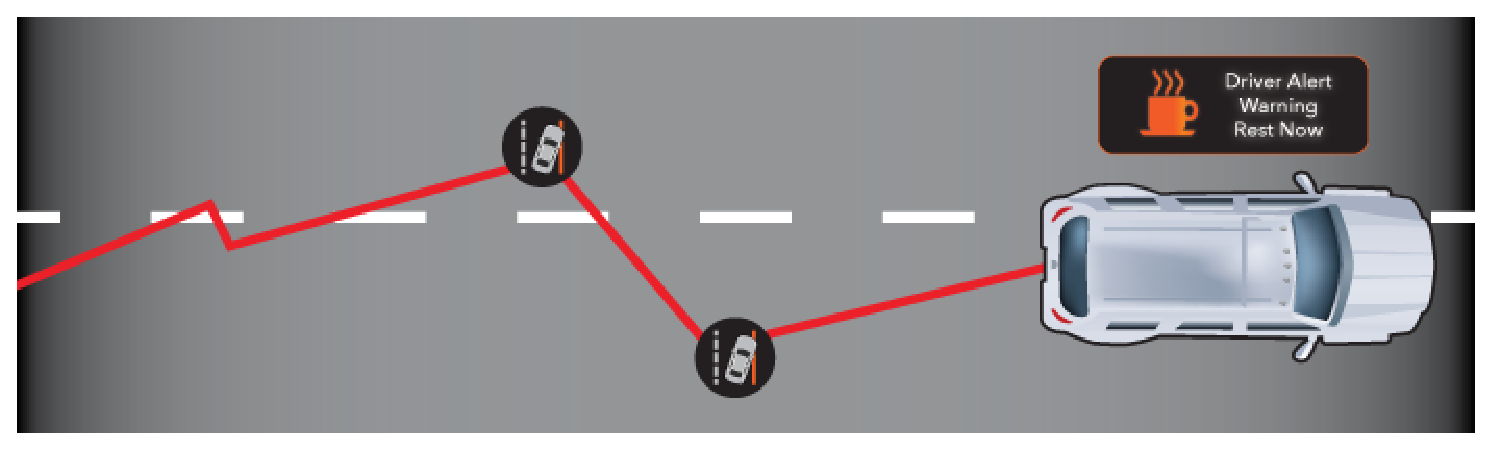
\includegraphics[width=.8\linewidth]{eps/sdlp.eps}
		\caption{Funzionamento della misura SLDP basata\\sul veicolo.}
	\end{subfigure}
	\begin{subfigure}{.4\textwidth}
		\centering
		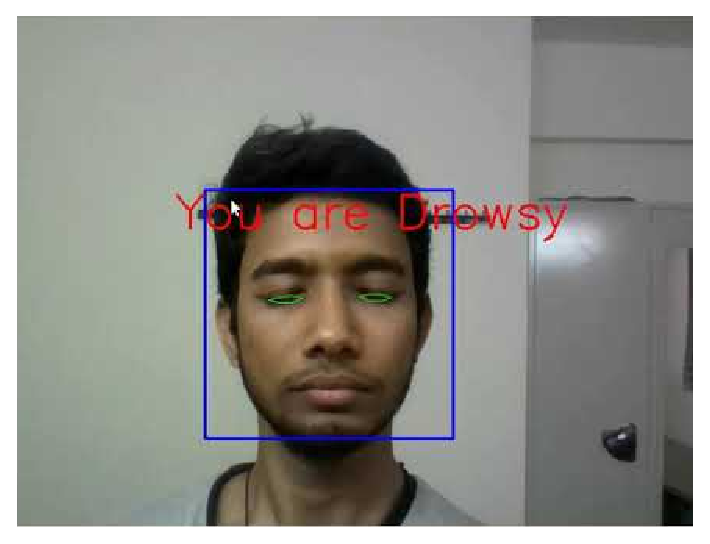
\includegraphics[width=.8\linewidth]{eps/ear.eps}
		\caption{Misure comportamentale incentrate sulla chiusura degli occhi calcolata con tecniche di Computer Vision.}
	\end{subfigure}
	\caption{Esempi di soluzioni per il rilevamento della sonnolenza alla guida, con distinzione nella misura adottata.}
	\label{fig:StateOfTheArt}
\end{figure}

\subsection{Confronto col progetto presentato}
Il progetto analizzato in questa relazione realizza il rilevamento della sonnolenza attraverso una misura comportamentale incentrata sulla chiusura degli occhi del conducente. Si basa pertanto su tecniche di Computer Vision sia per la \quotes{face detection} che per l'estrazione dei \quotes{facial landmark}. L'apertura degli occhi è calcolata mediante l'EAR, una soluzione diffusa in letteratura (come alternativa al PERCLOS) e nota per i suoi vantaggi: stima incentrata su una sola grandezza scalare, superamento dei risultati allo stato dell'arte su due dataset standard, e ricavabile attraverso una semplice formula da una sola immagine. L'adozione del Raspberry Pi 3 B come piattaforma hardware di riferimento vincola in misura maggiore rispetto alle soluzioni presentate l'applicabilità di algoritmi di visione, costringendo a considerare con massimo riguardo il trade-off tra accuratezza e velocità d'elaborazione (real-time per requisito).

\iffalse
Riassumere le soluzioni presenti in letteratura inerenti al problema in esame. Per ciascuna, discutere le principali diversità o affinità rispetto al progetto presentato. Nel caso non siano presenti soluzioni direttamente comparabili a quella presentata descrivere comunque le principali tecniche note per affrontare la tematica trattata.\\

Le soluzioni esposte devono essere corredate degli opportuni riferimenti bibliografici. Nel caso si tratti di soluzioni già operative sul mercato, devono essere indicate le fonti (online) dove poter accedere al servizio o approfondirne i contenuti.\\

Vincoli circa la lunghezza della sezione (escluse didascalie, tabelle, testo nelle immagini, schemi):

\vspace{1cm}
\begin{tabular}{l|rr}
 & Numero minimo di battute & Numero massimo di battute \\
 \hline
 1 componente & 2000 & 3000 \\
 2 componenti & 2500 & 4500 \\
 3 componenti & 3000 & 6000 \\
 \hline
\end{tabular}
\fi

\newpage


%----------------------------------------------------------------------------------------
%	ANALISI DEI REQUISITI
%----------------------------------------------------------------------------------------

\section{Analisi dei requisiti}

In questa sezione sono trattati in modo dettagliato tutti i requisiti del progetto, emersi durante la fase di analisi.

\subsection{Business Requirements}
\begin{enumerate}
	\item Realizzare un progetto di qualità sia nella sua parte software che hardware, valutandone accuratamente le prestazioni.
	\item Organizzare il lavoro in team, definendo un apposito piano e sperimentando la suddivisione di task mediante diagramma di Gantt.
	\item Mettere alla prova le conoscenze acquisite durante il corso relative ai sistemi embedded, al Raspberry Pi, alla videosorveglianza e alle tecnologie di sensing.
\end{enumerate}

\subsection{User Requirements}
\begin{enumerate}
	\item Possibilità di posizionare il dispositivo all'interno del veicolo, frontalmente al conducente.
	\item Capacità del sistema di riconoscere il livello di sonnolenza del guidatore, considerando una misura comportamentale basata sulla chiusura degli occhi.
	\begin{enumerate}
		\item Il sistema deve considerare il guidatore in uno stato di sonnolenza e pertanto in una situazione di pericolo se la chiusura dei suoi occhi si protrae per un tempo eccessivo.
		\item Nella misurazione della sonnolenza, il sistema deve tener conto della reale apertura di ambo gli occhi.
	\end{enumerate}
	\item Avvio automatico del sistema all'atto dell'alimentazione.
	\item Attivazione o disattivazione del rilevamento su richiesta del conducente.
	\begin{enumerate}
		\item Il sistema deve procedere al monitoraggio del volto del conducente, al rilevamento del suo grado di sonnolenza e alla segnalazione di scenari di pericolo solo se attivo.
	\end{enumerate}
	\item Gestione degli scenari d'uso legati al riconoscimento del volto.
	\begin{enumerate}
		\item Volto rilevato. Il sistema deve procedere con la misura dell'indice di sonnolenza.
		\item Volto non rilevato. Il sistema non deve produrre allarmi, evitando segnalazioni potenzialmente non connesse a situazioni di reale pericolosità.
	\end{enumerate}
	\item Segnalazione acustica e visiva degli scenari di pericolo rilevati.
\end{enumerate}

\subsection{Functional Requirements}
\begin{enumerate}
	\item Il sistema deve monitorare il viso dell'utente attraverso una camera.
	\item La misurazione della sonnolenza del conducente deve avvenire grazie a tecniche di Computer Vision.
	\begin{enumerate}
		\item Il sistema deve applicare tecniche di face recognition per l'individuazione del volto.
		\item Il sistema deve applicare tecniche di facial landmarking per l'individuazione delle sole coordinate di interesse per quanto concerne gli occhi.
		\item Il sistema deve rilevare la chiusura degli occhi nei vari frame grazie al calcolo dell'EAR per ognuno di essi.
		\item Si considera la presenza di uno scenario di pericolo nel momento in cui la misura dell'EAR indica la chiusura degli occhi per un definito numero di frame consecutivi, ritenuto di adatta sensibilità per gli obiettivi del sistema.
	\end{enumerate}
	\item Il sistema deve avviare il software di rilevamento nella fase di reboot.
	\item Il sistema deve consentire l'avvio o l'arresto della rilevazione mediante la pressione di un pulsante.
	\begin{enumerate}
		\item L'acquisizione dei frame dalla camera e la loro successiva elaborazione devono avvenire solo se il sistema è attivo.
	\end{enumerate}
	\item Il sistema deve adottare un comportamento idoneo sia a fronte del riconoscimento del volto che del fallimento di tale fase.
	\begin{enumerate}
		\item Volto rilevato. Il sistema deve procedere con l'estrazione dei facial landmark e il calcolo dell'EAR per entrambi gli occhi.
		\item Volto non rilevato. Il sistema deve procedere con l'analisi dei successivi frame, senza segnalare situazioni di pericolo.
	\end{enumerate}
	\item Il sistema deve segnalare al conducente la presenza di uno scenario di pericolo causato dal rilevamento di sonnolenza, adottando due tipologie distinte di avvertimento.
	\begin{enumerate}
		\item Avvertimento acustico, per mezzo di un buzzer sonoro.
		\item Avvertimento visivo, per mezzo di LED.
	\end{enumerate}
\end{enumerate}

\subsection{Non-functional Requirements}
\begin{enumerate}
	\item \textbf{Dimensioni.} Il sistema deve avere dimensioni conformi per una sua installazione a bordo di un autoveicolo, in modo da non ostacolare in alcun modo la guida. L'intera soluzione deve pertanto essere facile da trasportare e poco ingombrante.
	\item \textbf{Real-time.} Il sistema deve essere in grado di elaborare i frame catturati e di fornire segnalazioni di pericolo in tempo reale, specie in considerazione della velocità con cui il veicolo potrebbe essere in movimento. Ciò ha impatto sia sulla scelta dell'hardware - che deve risultare di sufficiente capacità computazionale - sia sulla progettazione del software - che non deve rivelarsi eccessivamente complesso nel rispetto delle limitate risorse che si hanno a disposizione sulla piattaforma scelta.
	\item \textbf{Affidabilità.} Il rilevamento della sonnolenza del conducente deve avvenire nel modo più accurato possibile, riducendo al minimo il numero di falsi positivi e consentendo solo ridotti margini di errore. Il sistema deve essere robusto a eventuali variazioni dell'ambiente, della luminosità e dell'orientamento del volto. Ove possibile, inoltre, l'oggettistica, gli indumenti indossati e la colorazione della pelle del guidatore non devono compromettere il funzionamento del sistema stesso.
\end{enumerate}

\subsection{Implementation Requirements}
\begin{enumerate}
	\item \textbf{Raspberry Pi 3 B}. La componente hardware del sistema deve essere basata su Raspberry Pi 3 B, un single-board computer economico, di ridotte dimensioni e di buone capacità computazionali. La ragione alla base di tale scelta è da ricercarsi nella volontà di approfondire le conoscenze apprese durante il corso di Smart City e Tecnologie Mobili, acquisendo anche esperienza nello sviluppo di progetti basati su questo tipo di piattaforma.
	\item \textbf{Budget}. La realizzazione del sistema deve avvenire a basso costo da un punto di vista economico in tutte le sue componenti, nell'ottica anche di un ipotetico deployment su larga scala.
\end{enumerate}

\iffalse
In questa sezione esporre brevemente i requisiti a cui il sistema proposto deve rispondere, concentrando l'attenzione sugli aspetti più rilevanti e facendo eventualmente uso di opportuni diagrammi di alto livello.\\

Vincoli circa la lunghezza della sezione (escluse didascalie, tabelle, testo nelle immagini, schemi):

\vspace{1cm}
\begin{tabular}{l|rr}
 & Numero minimo di battute & Numero massimo di battute \\
 \hline
 1 componente & 4000 & 6000 \\
 2 componenti & 6000 & 8000 \\
 3 componenti & 8000 & 10000 \\
 \hline
\end{tabular}
\fi


\newpage


%----------------------------------------------------------------------------------------
%	PROGETTAZIONE
%----------------------------------------------------------------------------------------

\section{Progettazione}

Devono essere esposte le scelte progettuali operate nelle varie fasi di sviluppo dell'elaborato.\\

In questa sezione devono essere documentati gli schemi di progetto relativamente all'architettura complessiva del sistema e alle sue componenti di rilievo che possano meritare un'analisi di dettaglio. Per le componenti software si può ricorrere ad esempio a diagrammi delle classi, di sequenza, stato, attività. Per le componenti hardware è possibile includere opportuni schemi in grado di descrivere l'architettura fisica adottata.\\

Vincoli circa la lunghezza della sezione (escluse didascalie, tabelle, testo nelle immagini, schemi):

\vspace{1cm}
\begin{tabular}{l|rr}
 & Numero minimo di battute & Numero massimo di battute \\
 \hline
 1 componente & 9000 & 18000 \\
 2 componenti & 12000 & 21000 \\
 3 componenti & 15000 & 24000 \\
 \hline
\end{tabular}


\newpage


%----------------------------------------------------------------------------------------
%	IMPLEMENTAZIONE
%----------------------------------------------------------------------------------------

\section{Implementazione}\label{sec:implementazione}

Esporre i principali problemi affrontati durante l'effettiva realizzazione delle componenti hardware/software e illustrare le soluzioni implementative adottate. Se l'elaborato ha previsto l'utilizzo di tecnologie già disponibili sul mercato, discuterne brevemente le caratteristiche e motivarne l'adozione rispetto ad altre soluzioni assimilabili.\\

\textbf{NOTA: in questa sezione devono essere riportate esclusivamente le porzioni di codice ritenute particolarmente significative. Il codice sorgente nella sua interezza, opportunamente commentato, deve essere consegnato separatamente dalla relazione in un archivio compresso.}\\


Vincoli circa la lunghezza della sezione (escluse didascalie, tabelle, testo nelle immagini, schemi):

\vspace{1cm}
\begin{tabular}{l|rr}
 & Numero minimo di battute & Numero massimo di battute \\
 \hline
 1 componente & 5000 & 11000 \\
 2 componenti & 8000 & 16000 \\
 3 componenti & 10000 & 21000 \\
 \hline
\end{tabular}


\newpage


%----------------------------------------------------------------------------------------
%	TESTING E PERFORMANCE
%----------------------------------------------------------------------------------------

\section{Testing e performance}

Esporre lo stato di funzionamento effettivo del sistema progettato ad elaborato concluso. Per ciascuna delle funzionalità salienti devono essere tabellate e discusse le performance riscontrate mediante opportuni test eseguiti in fase di validazione del progetto.\\

I tempi di esecuzione/comunicazione devono essere accompagnati dalle caratteristiche dell'hardware sul quale è eseguito il software.\\

Qualora l'elaborato includa algoritmi innovativi, indicarne la complessità computazionale (avendo cura di esporre lo pseudo codice nella sezione \ref{sec:implementazione}).\\


Vincoli circa la lunghezza della sezione (escluse didascalie, tabelle, testo nelle immagini, schemi):

\vspace{1cm}
\begin{tabular}{l|rr}
 & Numero minimo di battute & Numero massimo di battute \\
 \hline
 1 componente & 2000 & 3000 \\
 2 componenti & 2500 & 4500 \\
 3 componenti & 3000 & 6000 \\
 \hline
\end{tabular}


\newpage


%----------------------------------------------------------------------------------------
%	ANALISI DI DEPLOYMENT SU LARGA SCALA
%----------------------------------------------------------------------------------------

\section{Analisi di deployment su larga scala}

In questa sezione va discussa, eventualmente con l'ausilio di opportuni diagrammi (componenti, deployment), l'evoluzione del progetto presentato immaginando che venga adottato su larga scala. I dettagli qui esposti devono quindi astrarre dalle specifiche dell'elaborato qualora l'implementazione sia stata focalizzata su uno scenario isolato.\\

A titolo d’esempio, qualora applicabile, devono essere evidenziate le criticità che si potrebbero incontrare e devono essere proposte soluzioni tipiche in contesti di \textit{cloud architecture} per garantire un'adeguata \textit{resilienza}, in termini di \textit{availability} e \textit{scalability} del sistema.\\


Vincoli circa la lunghezza della sezione (escluse didascalie, tabelle, testo nelle immagini, schemi):

\vspace{1cm}
\begin{tabular}{l|rr}
 & Numero minimo di battute & Numero massimo di battute \\
 \hline
 1 componente & 3000 & 6000 \\
 2 componenti & 4500 & 9000 \\
 3 componenti & 6000 & 12000 \\
 \hline
\end{tabular}


\newpage


%----------------------------------------------------------------------------------------
%	PIANO DI LAVORO
%----------------------------------------------------------------------------------------

\section{Piano di lavoro}

In questa sezione devono essere chiariti i compiti svolti da ciascun candidato nel caso in cui il gruppo abbia più di un componente.\\

Deve essere inoltre esposto il piano di lavoro adottato. A tal fine, per ogni attività svolta durante la preparazione dell'elaborato (ad esempio: studio di una tecnologia, progettazione di un componente, implementazione di un algoritmo ecc…) deve essere chiarita la collocazione temporale e devono essere indicate le risorse impiegate per svolgerla (giorni/uomo). I candidati possono ricorrere a opportuni diagrammi come quello di Gantt.\\


Vincoli circa la lunghezza della sezione (escluse didascalie, tabelle, testo nelle immagini, schemi):

\vspace{1cm}
\begin{tabular}{l|rr}
 & Numero minimo di battute & Numero massimo di battute \\
 \hline
 1 componente & 1000 & 2000 \\
 2 componenti & 1500 & 3000 \\
 3 componenti & 2000 & 4000 \\
 \hline
\end{tabular}

\newpage


%----------------------------------------------------------------------------------------
%	CONCLUSIONI
%----------------------------------------------------------------------------------------

\section{Conclusioni}

However, it has been found that the rate of detecting the correct feature, or the percentage of success among a number of detection attempts, varies depending on the application and number of classes. The determination of drowsiness using PERCLOS and Eye Blink has a success rate of close to 100\% [43] and 98\% [45], respectively. However it has to be noted that, the high positive detection rate achieved by [43] was when the subjects didn’t wear glasses. Likewise, as most researchers conducted their experiments in simulated environment they achieved a higher success rate. The positive detection rate decreased significantly when the experiment was carried out in a real environment [15].
Another limitation of behavioral measure was brought out in an experiment conducted by Golz et al. They evaluated various drowsiness monitoring commercial products, and observed that driver state cannot be correlated to driving performance and vehicle status based on behavioral measures alone [57].

Esporre brevemente le considerazioni conclusive sul progetto presentato, indicando anche i possibili sviluppi futuri.\\

Vincoli circa la lunghezza della sezione (escluse didascalie, tabelle, testo nelle immagini, schemi):

\vspace{1cm}
\begin{tabular}{l|rr}
 & Numero minimo di battute & Numero massimo di battute \\
 \hline
 1 componente & 500 & 1000 \\
 2 componenti & 1000 & 2000 \\
 3 componenti & 1500 & 3000 \\
 \hline
\end{tabular}

\newpage


%----------------------------------------------------------------------------------------
%	APPENDICE
%----------------------------------------------------------------------------------------

\appendix
\addcontentsline{toc}{section}{Appendice}
\section*{Appendice}
Laddove necessario è possibile avvalersi di appendici alla relazione per includere materiale di approfondimento.\\

A titolo esemplificativo possono essere incluse le schede tecniche dei componenti adottati, la normativa di riferimento che regola un particolare dominio applicativo, ecc.


\newpage


%----------------------------------------------------------------------------------------
%	RIFERIMENTI BIBLIOGRAFICI
%----------------------------------------------------------------------------------------

\bibliography{relazione}
\bibliographystyle{unsrt}

%----------------------------------------------------------------------------------------

\end{document}